%MIT OpenCourseWare: https://ocw.mit.edu
%RES.18-011 Algebra I Student Notes, Fall 2021
%License: Creative Commons BY-NC-SA 
%For information about citing these materials or our Terms of Use, visit: https://ocw.mit.edu/terms.

% \section{Finite subgroups of \texorpdfstring{$SO_3$}{SO3}}

\section{Stabilizer}

\subsection{Review}
A group action is when a group $G$ acts on a set $S$ by 
\[
G \by S \rto S
\]
and sends
\[
(g, s) \mto gs.
\]

The orbit of an element in $s$ is all the elements it gets mapped to,
\[
O_s = \{gs \in S : g \in G\},
\]
and the stabilizer is 
\[
\stab_G(s) \coloneqq \{g \in G: gs = s\} \leq G,
\]

\subsection{Counting Formula}
\begin{figure}[h]
    \centering
    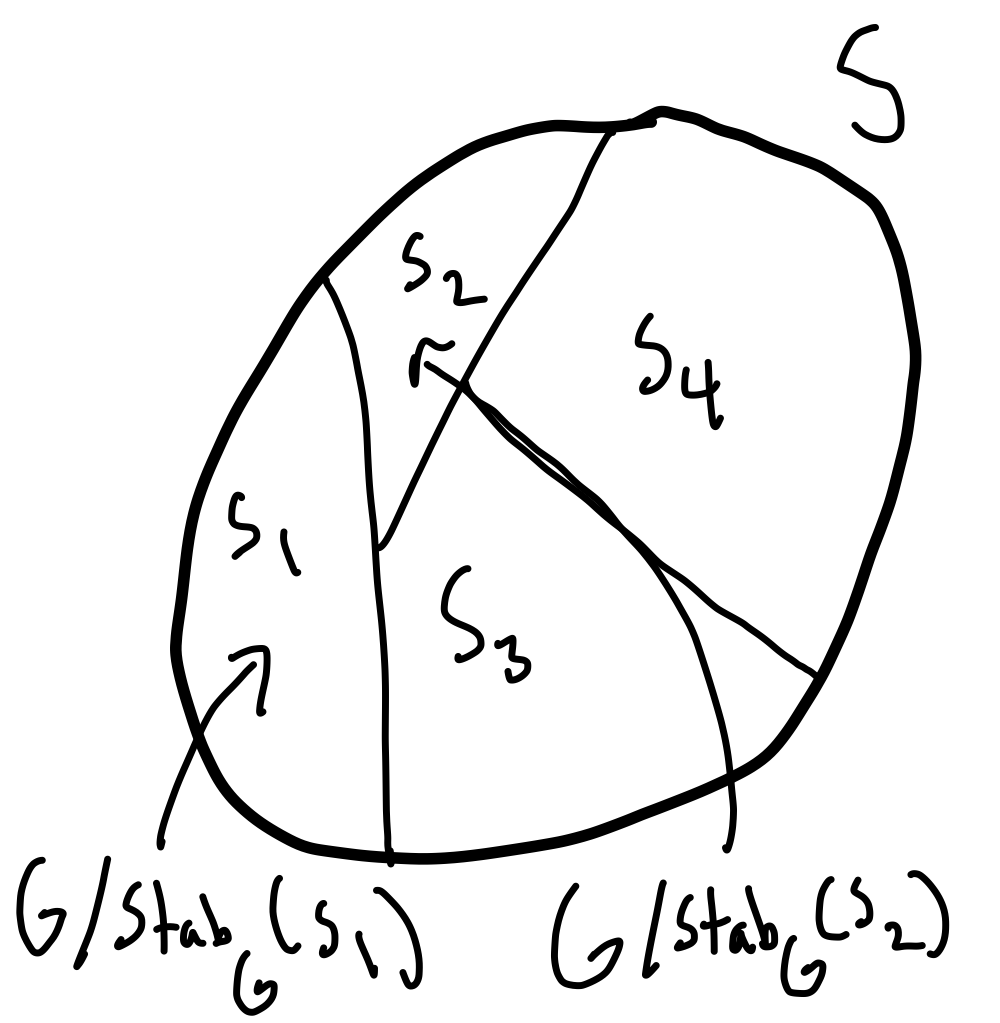
\includegraphics[width=6cm]{Lecture Files and Images/lec18-orbits.png}
    \caption{The partition of $S$ into orbits and theeir corresponding bijections with $G/\stab(s_i)$}
\end{figure}

One of the facts we learned about orbits is that they partition $S$. 
We further learned that there is a bijection between the left cosets of the stabilizer with the orbit.
We were then able to write the size of $S$ as 
\[
|S| = \sum |O_{s_i}| = \sum [G: \stab(s_i)].
\]


\subsection{Stabilizers of Products}
Given a group $G$ acting on a set $S$ and an element $s\in S$, we know that $|O_s| = [G:\stab(s)].$
This also means that we expect that if we take the stabilizer of two elements in the same orbit, then they should be the same size. Specifically, we are asking what can we say about the stabilizer of a product. If $s' = as$ for $a \in G,$ if $g \in \stab(s),$ then $gs = s.$ 
Then 
\[
aga^{-1}(s') = aga^{-1}(as) = ag(s) = as = s'.
\]
In other words, if $g$ stabilizes $s$, then $aga^{-1}$ stabilizes $s'$. 
So the upshot is that 
\[
\stab_G(s') = a\stab_G(s)a^{-1}.
\]
If $\stab_G(s')$ was normal, then the two stabilizers would be the same, but this doesn't have to be the case. 
We've provided a nice bijection to see that the sizes of the two stabilizers must be the same size.
\subsection{Statement}
Today, we will look at a consequence of these counting formulae.
Recall that we were able to study and classify finite and discrete subgroups of isometries in the plane. 
The special orthogonal group $SO_3$ is the group of rotations $\rho_{(u, \theta)}$ in $\RR^3$ fixing $\vv{0}$. What are the finite subgroups $G \leq SO_3$?

In fact, there are not so many! Let's start with the theorem.
\begin{theorem}
If $G \leq SO_3$, then 
\begin{itemize}
    \item $G \cong C_n = \langle \rho_{u, 2\pi/n}\rangle$, or
    \item $G \cong D_n = \langle \rho_{u, 2\pi/ n}\rangle$, or 
    \item $G$ is the group of rotational symmetries of a regular polyhedron.
\end{itemize}
\begin{figure}[H]
    \centering
    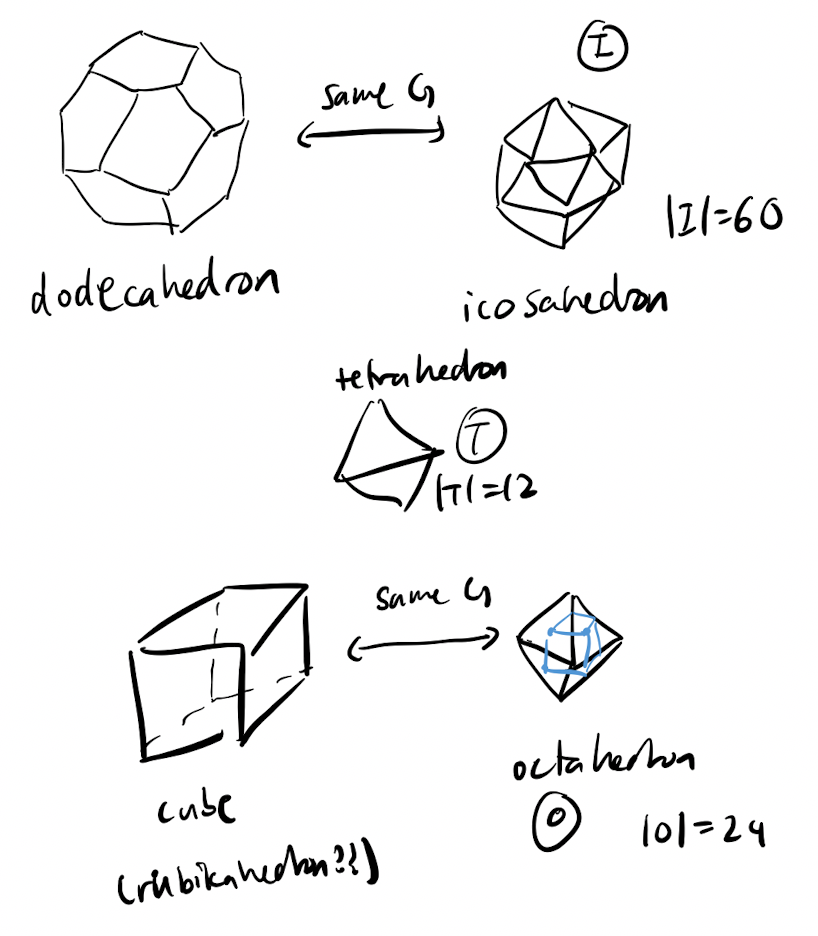
\includegraphics[width=10cm]{Lecture Files and Images/lec18-hedra.png}
    \caption{The regular polyhedra}
\end{figure}

\end{theorem}
Although there are 5 regular polyhedra, there are only 3 distinct subgroups of symmetries. 
The dodecahedron and icosahedron have the same symmetries, which we denote as $I$.
The cube and octahedron have the same symmetries as well, which we denote by $O$.
Finally, the tetrahedron is partnered with itself and we denote its symmetries with $T$.

As an example to see why some of the symmetries are the same, consider the symmetries of the octahedron. 
We can draw a point on the center of every face in the octahedron. 
Connecting these points lead to a cube, and thus any rotational symmetry of the cube will give a symmetry of the octahedron, and vice versa. 
A similar argument can be applied to the dodecahedron and icosahedron.
Trying the argument for a tetrahedron just maps to the tetrahedron itself.

On Wednesday, we worked out that the group of symmetries of a cube has size 24. Similarly, the tetrahedron has $|T| = 12,$ and $|I| = 60.$

%9:08
We will prove this by studying orbits! An non-identity element $g \neq I \in G$\footnote{We use $I$ for the identity here} is a rotation and thus fixes two unit vectors, which are exactly the positive and negative unit vectors on the rotation axis of $g$. These are called the \emph{poles} of $g.$ Let 
\[
\mathcal{P} = \bigcup_{g \neq I} \{\text{poles of }g\}.
\]

\begin{lemma}
If $p \in \mathcal{P}$ and some $g \in G,$ then $gp \in \mathcal{P}$ also. As a result, we learn that $G$ acts on $\mathcal{P}$. 
\end{lemma}

\begin{proof}
For $p \in \mathcal{P}$, then there exists $h \neq I \in G$ such that $hp = p.$ If $p' = g(p).$ Then $ghg^{-1}(p') = p'$ by earlier reasoning. Then $ghg^{-1} \in G$, and $ghg^{-1}\neq I$ since $h \neq I.$ thus $p' \in \mathcal{P}$ also.
\end{proof}

\begin{example}
\label{CyclicPoles}
Let $G = C_n$. Then $\mathcal{P} = \{p, -p\}$ since every rotation will have the same poles.
\end{example}

\begin{example}
\label{PolyhedraPoles}
Let $G = O.$\footnote{The group of symmetries of an octahedron.} Then $\mathcal{P} = \{\text{pole for each vertex, edge, or face}\}.$ %14:53
\end{example}

Now, what can we say about stabilizers of these subgroups. let $|G| = N.$ Let's decompose $\mathcal{P}$ into orbits. Then $\mathcal{P} = \mathcal{O}_1 \cup \mathcal{O}_2 \cup \cdots \cup \mathcal{O}_k$. Then $|\mathcal{O}_i| = n_i,$ and $\mathcal{O}_i = \mathcal{O}_{p_i}$ for some pole $p_i$. Then by our relations about the number of index of the stabilizer
\[
|\stab(p_i)| = r_i = \frac{N}{n_i}.
\]
Note that the stabilizer group will be a cyclic group.
Geometrically, it will just contain the rotations around the axis $p_i$.

\subsection{Finding the subgroups}

Let's write down an auxiliary set. It is the set of poles \emph{and} group elements paired together. Let 
\[
S \coloneqq \{(g, p), g \neq I, p \text{ is a pole for }g\}.
\]

Then we can count the order of $S$ in two different ways. 

The order of $S$ is
\[
|S| = \sum_{\substack{g \in G\\ g \neq I}} 2 = 2(N-1),
\]
since there are two poles for every non-identity element of $G.$

Additionally, since we have $k$ orbits,
\[
|S| = \sum_{p \in \mathcal{P}} |\stab(p)|  - 1 = \sum_{i = 1}^k n_i(r_i - 1) = \sum_{i=1}^k \frac{N}{r_i}(r_i - 1).
\]

Every pole in the same orbit has the same stabilizer size, so we can group them together.
Now, we have that 
\[
\sum_{i = 1}^k \frac{N}{r_i}(r_i-1) = 2(N-1). 
\]

Dividing by $N,$
\[
\left(1 - \frac{1}{r_1}\right) + \left(1 - \frac{1}{r_2}\right) + \cdots + \left(1 - \frac{1}{r_k}\right) = 2 - \frac{2}{N}.
\]

Each of these quantities $1 - \frac{1}{r_1}$ is between $1/2$ and $1,$ since $r_1$ must be at least two (by the definition of a pole.) %??
So $1 - \frac{1}{r_1} \in \left[\frac{1}{2}, 1\right).$

In addition $2 - \frac{2}{N} \in [1, 2).$ So $k = 2$ or 3, since this is the only way the counting formula works out from our bounds. 
In fact, this works out for examples \ref{CyclicPoles} and \ref{PolyhedraPoles}. 
For $G=C_n$, we have two orbits, and for $G=O$ we have three orbits, even though it is much more complicated.

For $k = 2,$ when there are two orbits, 
\[
1 - \frac{1}{r_1} + 1 - \frac{1}{r_2} = 2 - \frac{2}{N},
\]
and so
\[
\frac{1}{r_1} + \frac{1}{r_2} = \frac{2}{N}.
\]
But since $r_1, r_2 \leq N,$ 
\[
\frac{2}{N} \leq \frac{1}{r_1} + \frac{1}{r_2} = \frac{2}{N}.
\]

We have $r_1 = r_2 = N,$ and $n_1 = n_2 = 1.$ Each of the poles is fixed by the \emph{entire} group. Then $G$ is a finite subgroup of $SO_2,$ and thus $G = C_N,$ a cyclic subgroup.

For the three-orbit case, the numerics of the problem is also extremely constraining. When $k = 3,$ the equation is 
\[
1 - \frac{1}{r_1} + 1 - \frac{1}{r_2} + 1 - \frac{1}{r_3} = 2 - \frac{2}{N},
\]
and equivalently 
\[
\frac{1}{r_1} + \frac{1}{r_2} + \frac{1}{r_3} = 1 + \frac{2}{N}.
\]
Without loss of generality, let $r_1 \leq r_2 \leq r_3.$ It is necessary for $r_1 = 2,$ or else the LHS\footnote{left hand side} would be $\leq 1.$ If $r_2\geq 4,$ then $r_3 \geq 4$ as well, and again the LHS would be $\leq 1.$ So $r_2 = 2$ or $3.$ Finally, if $r_2 = 3,$ then $r_3$ cannot be $\geq 6,$ again from the numerics of the problem. So $r_3 = 3, 4,$ or 5. 

In total, the cases are 
\begin{itemize}
    \item \textbf{Case 1.} $(2, 2, r):$ $r = N/2$. In this case, we still have an infinite family. 
    \item \textbf{Case 2.} $(2, 3, 3)$. We can solve for $N$ to get $N = 12.$ This corresponds to the tetrahedral group $T.$
    \item \textbf{Case 3:} $(2, 3, 4)$. $N = 24$. This corresponds to the octahedral group $O.$
    \item \textbf{Case 4:} $(2, 3, 5)$. $N = 60.$ This corresponds to the icosahedral group $I.$
\end{itemize}

We can really \emph{strongly} limit the possibilities of a group $G$. We got this by counting a set $S$ in two different ways, and playing around with the numbers and fractions. %30:21

We aren't done; we still have to show that these cases \emph{actually} correspond to the groups. In each of these cases, we have three orbits, and those correspond to edges, faces, and vertices of these regular polyhedra. The pole for any vertex can be rotated to the pole for any other vertex. We'll do the argument for the octahedral group and it will be similar for the remaining polyhedra.

\subsection{The Octahedral Group}
\begin{example}[Octahedral group]
Let's take (2, 3, 4) and argue that this group \emph{must} be symmetries of a cube or an octahedron. For $4,$ $n_3 = 6.$ So the stabilizer has size 4 and the orbit has size 6. Let's try to figure out what the orbit looks like. It contains six vectors inside $\RR^3,$ so we can simply see the possible configurations. 

Drawing the first vector is easy; we just pick wherever we want for $p.$ Then $-p$ has to be in the same orbit as well because $\stab_G(-p)$ has the same order as $\stab_G(p),$ but we only have one orbit with stabilizer size 4. What does the stabilizer group look like? Geometrically, it's rotations around $p$ and must have size 4, so we have $\stab_g(p) = C_4.$ 
\begin{center}
    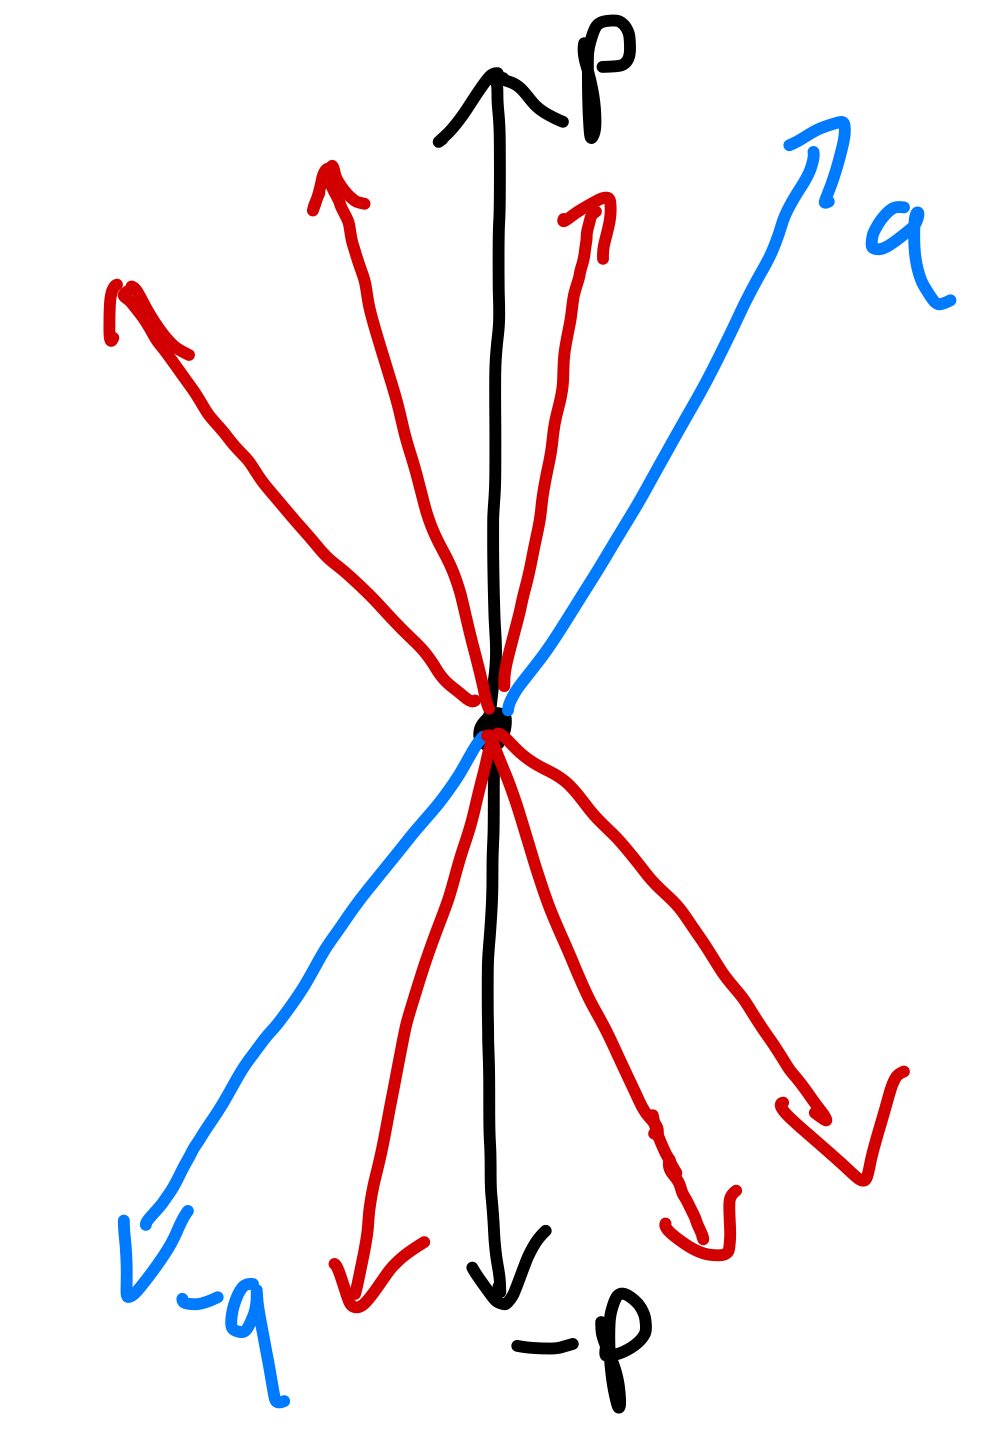
\includegraphics[width=4cm]{Lecture Files and Images/lec18-wrongpoles.png}
\end{center}
Now, let's try to figure out the other 4 poles in our orbit. Suppose we draw $q$ such that $p$ and $q$ are not perpendicular.
For any $q$ in the orbit, $-q$ is also in the orbit. We have determined that rotations by $\pi/2$ around $p$ are in our group, so those rotations of $q$ should also be in our orbit. However, this gives us 4 vectors for rotations of $q$ and 4 vectors for rotations of $-q$, and this is too many. 
This picture was wrong because $q$ was not drawn perpendicular to $p.$ If we drew $q$ perpendicular, then rotating $q$ by 90 degrees gives us an orbit of size 6. 

\begin{center}
    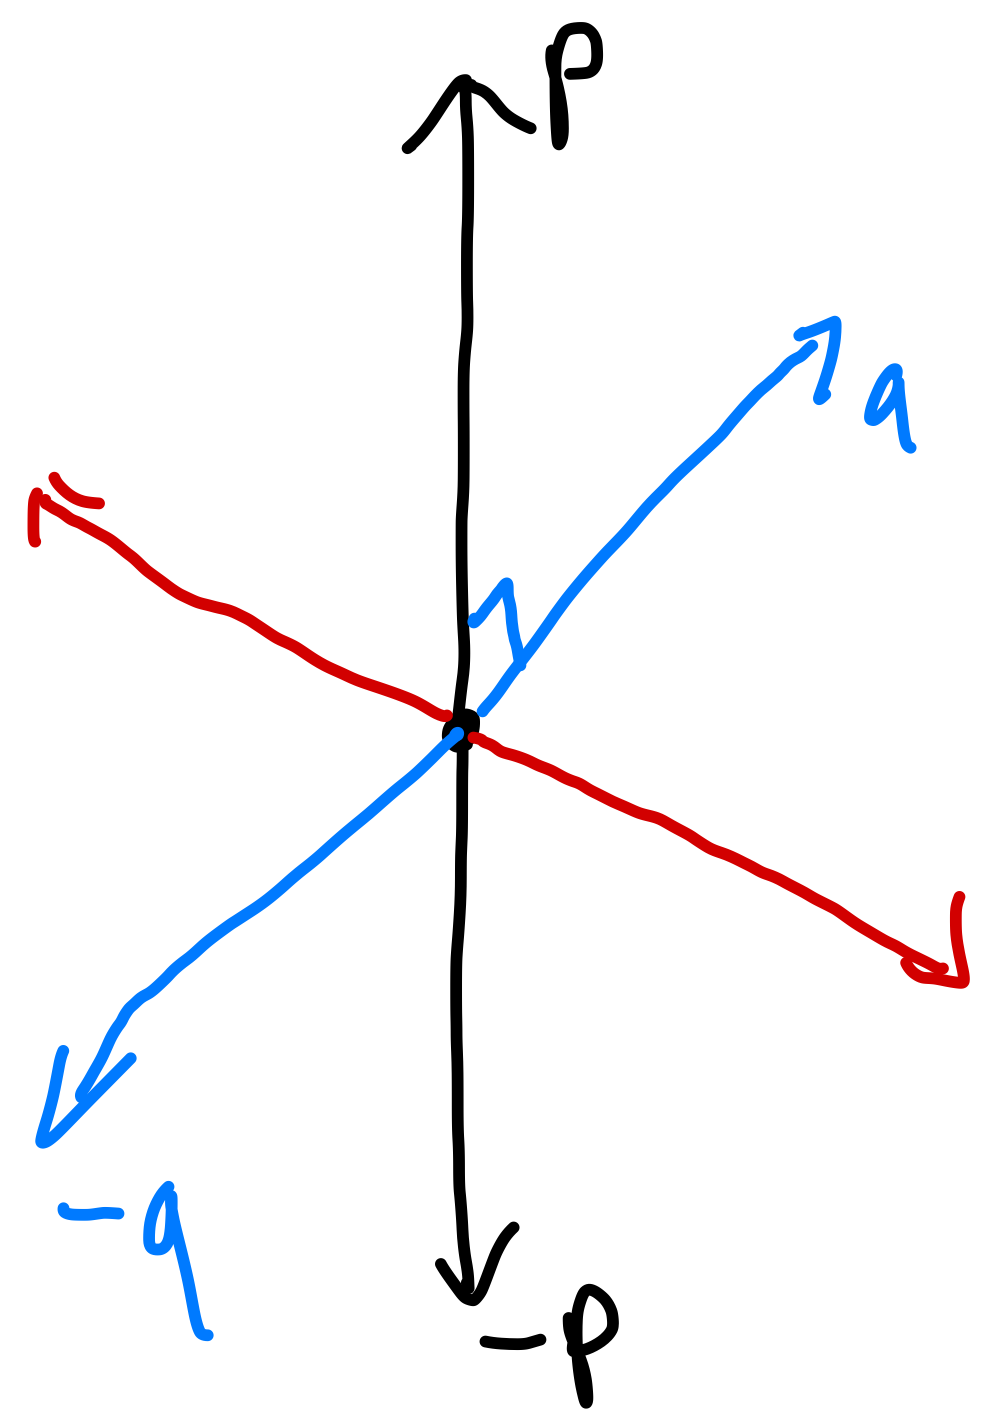
\includegraphics[width=4cm]{Lecture Files and Images/lec18-rightpoles.png}
\end{center}
Whatever the group $G$ is, it fixes the collection of vectors that we drew. In particular, it fixes the octahedron obtained by taking the convex hull of the vectors and thus $G\leq O$. But the octahedral group has size 24\footnote{we worked this out in class on Wednesday} and this group also has size 24, so $|G| = |O| = 24$ implies that $G = O.$

%37:11
\end{example}

We can repeat this for all the cases to finish the proof, but it isn't too important. 
The key lesson is how we were able to use the counting formulas and orbit decomposition of the set to really constrain the possibilities in these ways.
A lot of the challenge was just finding the right set to act on; in this case it was the poles. 

% \begin{question}[Student Question]
% The number of discrete symmetry group s is less than the number of Platonic solids; this is because some of the polyhedra have the same symmetry groups! For example, the dodecahedron and the icosahedron have the same symmetry group $G;$ this is because they are "duals" of each other by replacing faces by vertices. Did this just happen as a coincidence or is there any way to predict it?
% \end{question}
% ethany: idk lol
\newpage